\documentclass{article}
\usepackage{graphicx}
\usepackage{amsmath,amssymb,enumerate,graphicx,pgf,tikz,fancyhdr}
\usepackage{geometry}
\usepackage{tabvar}
\usepackage{fontspec}
\usepackage{dot2texi}
\usepackage{hyperref}
\usepackage{minted}

\usetikzlibrary{backgrounds}
\usetikzlibrary{arrows.meta}
\usetikzlibrary{shapes.geometric}

\graphicspath{ {./images/} }
\title{\centering PERT Maker: Manuel d'utilisation}

\date{9 Novembre 2023}
\renewcommand{\contentsname}{Table des Matières}

\renewcommand{\theFancyVerbLine}{
    \sffamily\textcolor[rgb]{0.5,0.5,0.5}{\scriptsize\arabic{FancyVerbLine}}}
    
    
\begin{document}
    
    
\csundef{listing}\csundef{endlisting}
\csundef{listing*}\csundef{endlisting*}\maketitle
\tableofcontents{}
\newpage

\section{Présentation de PERT Maker}
\subsection{La méthode PERT}
PERT Maker est une solution logicielle d'utilisation de la méthode PERT de gestion de projet. \\
La méthode PERT fournit une méthode et des moyens pratiques pour décrire,
représenter, analyser et suivre de manière logique les tâches et le réseau des tâches à réaliser dans le cadre d'une 
action à entreprendre ou à suivre. \\
Un graphe de dépendances dépendances des tâches est notamment utilisé. \\
Pour chaque tâche sont indiquées une date de début au plus tôt, fin au plus tôt et fin au plus tard.  \\
Le graphe permet aussi de déterminer le chemin critique qui conditionne la durée minimale du projet.
Le but est de trouver la meilleure organisation possible pour qu'un projet soit terminé dans les délais, et d'identifier les tâches critiques, 
c'est-à-dire les tâches qui ne doivent souffrir \textbf{d'aucun retard} sous peine de retarder l'ensemble du projet.
(\textcolor{blue}{\href{https://fr.wikipedia.org/wiki/PERT}{Plus d'informations sur la méthode PERT}})


\subsection{Objectif de PERT Maker}

L'application PERT Maker a pour objectif de faciliter la gestion de projet. PERT Maker réalise un traitement intelligent de l'organisation de votre projet, suivant 
la méthode PERT, et vous en fournit un rapport complet, comprenant:
\begin{itemize}
    \item Un graphe permettant de visualiser la dépendance des taches
    \item Analyse de la faisabilité du projet
    \item Visualiser le chemin critique, c'est à dire le chemin des tâches qui doivent être faite dans le temps indiqué sous peine de retarder tout le projet.
    \item Visualiser l'historique du projet via 3 comptes rendus d'éxécution possibles.
\end{itemize} 
Vous devez donc suivre correctement ce manuel pour tirer le plein potentiel de PERT Maker!

\section{Conception de fichiers pour PERT Maker}
Le fichier de votre projet doit suivre plusieurs règles strictes pour être correctement analysé par PERT Maker.

\subsection{Le format CSV}
Votre fichier doit être au format CSV (Comma Separated Values)
Il s'agit d'un format de fichier texte, ou les données sont séparées par des virgules.
Il peut aussi être vu sous forme tabulaire.
Pour générer un fichier CSV, vous pouvez utiliser votre logiciel de tableur préféré:
Microsoft Excel, Google Sheets,LibreOffice, OpenOffice Calc, tous sont capables d'importer
et exporter des fichiers CSV.
Il vous suffit de choisir l'option CSV lors de l'exportation (ou enregistrement) de votre fichier.

\newpage
\subsection{Comment formater vos fichiers CSV?}
Pour assurer le bon déroulement de l'analyse de votre projet, votre fichier CSV doit impérativement suivre des règles précises.\\ \\
Pour vous accompagner dans l'utilisation de PERT Maker, vous avez à disposition dans le dossier de ce manuel un fichier \textbf{template.csv}. Nous vous conseillons de concevoir votre fichier de projet
à partir de la template et de ce manuel. 
\\ 
Voici un exemple de fichier au bon format (projet fictif de production de film):
\\
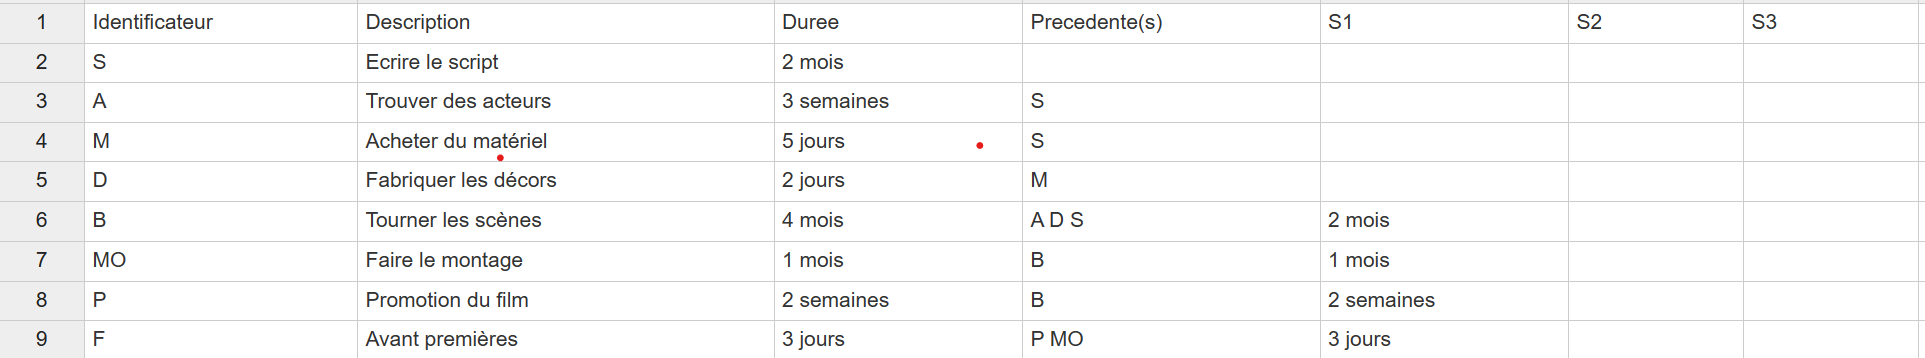
\includegraphics[scale=0.5]{csv_exemple}
\\
Tout d'abord, votre fichier doit contenir \textbf{au moins 4 colonnes, dont les noms sont standardisés}.\\
Les 4 premières sont réservées aux informations initiales du projet,
Toutes les suivantes vous permettent d'établir des comptes rendus d'éxécution, afin
de tenir compte de l'avancement du projet. \\
Chaque ligne correspond à une tâche. \\
Voici l'intêret et les règles de rédaction de chaque colonne : \\
\begin{itemize}
    \item Colonne 1 : Identificateur. L'abréviation du nom de la tâche. C'est ce nom qui sera utilisé dans le graphe de tâches. \textbf{Chaque abréviation doit être unique, et la dernière tâche doit obligatoirement être abréviée F.}
    \item Colonne 2 : Description.  La description précise de la tâche.
    \item Colonne 3 : Durée. La durée de la tâche. Les unités possibles sont jour(s), semaine(s), moi(s). \textbf{Attention à l'orthographe.}
    \item Colonne 4 : Précédente(s). Les abréviations de toutes les tâches nécéssaires au début de la tâche, \textbf{séparées d'un espace.}
    \item Colonne 5 et plus : Les différents suivis (comptes rendus d'éxécution). Contient la \textbf{durée restante de la tâche}, au même format que la colonne 4. \textbf{Si la tâche est terminée, laissez la case vide.}
\end{itemize}

\textbf{\textcolor{red}{Attention: Votre projet doit impérativement comporter une unique tâche finale. Elle doit représenter la fin du projet.
Si le projet se termine par plusieurs tâches parallèles, ajoutez une tâche finale qui admet toutes les dernières tâches dans la colonne
4 (Précédentes), avec une durée nulle.}}
\newpage
\subsubsection{Comment nommer vos fichiers projets?}
Il est préférable de ne pas utiliser d'espaces dans le noms de vos fichiers projets.\\

\subsection{Où placer vos fichiers projets ?}
Une fois votre fichier projet correctement crée et formaté, il suffit de le placer dans
le sous-dossier \textbf{Projets} du dossier de l'application. \\ Il pourra ainsi être reconnu
par PERT Maker. \\


\section{Utilisation de PERT Maker}
\subsection{Où et comment lancer PERT Maker ?}
Il suffit simplement d'éxécuter le fichier "PERT Maker.exe" présent dans le dossier de l'application.
\subsection{Que faire une fois PERT Maker en cours d'éxécution ?}
PERT Maker s'éxécute dans une fenêtre d'invite de commandes.
La liste des fichiers disponibles est immédiatement affichée.
Il suffit alors de donner le nom du fichier à analyser. \textbf{La casse est prise en compte.}\\
Vous devez ensuite préciser quelles informations analyser.\\
Si les colonnes dédiées aux suivis sont vides, elles seront ignorées.\\
Vous pouvez aussi choisir d'analyser chaque colonne séparément.\\
PERT Maker vous informera du déroulé de l'analyse.\\
Si une erreur se produit, elle vous sera détailée.

\section{Obtenir et exploiter vos analyses.}
\subsection{Où sont mes analyses ?}
Les résultats de l'analyse de vos projets par PERT Maker sont situées dans le sous-dossier
''\textbf{Analyses}'' du dossier de l'application. \\
Il contient lui même un sous dossier de l'Historique de chaque projet analysé par l'application.\\
Au sein du dossier Historique d'un projet, vous pouvez retrouver toutes les analyses demandées.
\subsection{Comment exploiter les fichiers d'analyse?}
PERT Maker produit des fichiers .tex .
Il s'agit de fichiers écrit dans le langage de compositions de documents \textcolor{blue}{\href{https://fr.wikipedia.org/wiki/LaTeX}{\LaTeX}}. \\ 
Cependant, vous pouvez facilement les convertir en fichier PDF, grâce à l'outil en ligne \textcolor{blue}{\href{https://www.overleaf.com/}{Overleaf}}.\\
Il vous suffit de créer un compte gratuit, puis un projet vide. Enfin, vous pouvez directement importer
vos fichiers .tex , et les compiler en PDF.
Si vous rencontrez des difficultés, voici un \textcolor{blue}{\href{https://shorturl.at/ersu1}{guide détaillé}}
sur cette procédure.\\
Alternativement, si vous disposez d'une distribution TeX telle que MikTex sur votre ordinateur,
vous pouvez directement compiler les fichiers, sans passer par Overleaf.

\section{Que faire en cas d'erreur non résolue?}
Si vous rencontrez un bug, ou une erreur persistante, n'hésitez pas a contacter le support ,à l'adresse suivante :
pertmakersupport@gmail.com
\end{document}